本研究では, 第4章で述べたシミュレーション環境を用いて3種類の
シミュレーション実験を行った. いずれの実験でも, 以下の3パターンを調べた. 
\begin{itemize}
  \item 認証機構を用いない場合
  \item ECDSAを用いて認証機構を追加した場合
  \item EdDSAを用いて認証機構を追加した場合
\end{itemize}

EdDSAのセキュリティ性能, ネットワークへの負荷, 計算効率を評価するために, 
次の8項目を評価基準とした. なお, どの項目も集計したデータの平均値を用いる.  
\vspace{-3mm}
\setlength{\columnsep}{10pt} % デフォルトは約35pt
\begin{multicols}{2}
  \begin{enumerate}
      \item スループット(TP)
      \item 遅延時間 (DT) 
      \item パケット配送率 (PDR)
      \item オーバーヘッドサイズ (OH)\\
      \item シミュレーション実行時間
      \item 署名作成時間
      \item 署名検証時間
      \item メモリ使用量
  \end{enumerate}
\end{multicols}
\begin{enumerate}
  \item \textbf{スループット(TP)}\\
  \indent \textbf{スループット}とは, 単位時間あたりに正常に転送された
  データ量のことである. 以下に示す式で定義される. ここで, 
  $AllTxBytes$は合計転送バイト数, $TxTimes$は
  転送にかかった時間である. \\
  \[
    TP = \frac{AllTxBytes\times 8}{TxTimes\times 1000}\text{[kbps]}
  \]
  \item \textbf{遅延時間(DT)}\\
  \indent \textbf{遅延時間}とは, パケットが送信されてから受信されるまでの
  時間のことである. 以下に示す式で定義される. ここで,
  $TxPacketTime$は送信ノードがパケットを送信した時間, 
  $RxPacketTime$は宛先ノードがパケットを受信した時間である. \\
  \[
    DT = RxPacketTime - TxPacketTime \text{[ms]}
  \]

  \item \textbf{パケット配送率(PDR)}\\
  \indent \textbf{パケット配送率}とは, 送信されたデータ量のうち
  損失せずに受信されたデータ量の割合のことである. 以下に示す式で定義される. 
  ここで, $AllTxPackets$は合計送信パケット数, $AllRxPackets$は
  合計受信バイト数である. \\
  \[
    PDR = \frac{AllRxPackets}{AllTxPackets} \times 100 \text{[\%]}
  \]

  \item \textbf{オーバーヘッドサイズ(OH)}\\
  \indent \textbf{オーバーヘッドサイズ}とは, データの送受信に付随して発生する
  余分なコストのことであり, ここではルーティングに使用される
  通信データ量を指す. 以下に示す式で定義される. ここで, 
  $AllTxKBytes$はHelloパケットを含めた全ノードの合計送信キロバイト数, 
  $TxKBytes$はデータパケットの合計送信キロバイト数である. \\
  \[
    OH = AllTxKBytes - TxKBytes \text{[KB]}
  \]

  \item \textbf{シミュレーション実行時間}\\
  \indent \textbf{シミュレーション実行時間}とは, 現実時間で5分間分のSUMOデータを使って
  1回のシミュレーションを行ったときの実行時間のことである. 

  \item \textbf{署名作成時間}\\
  \indent \textbf{署名作成時間}とは, データに署名を付与する際にかかった実時間のことである. 

  \item \textbf{署名検証時間}\\
  \indent \textbf{署名検証時間}とは, データの署名を検証する際にかかった実時間のことである.

  \item \textbf{メモリ使用量}\\
  \indent \textbf{メモリ使用量}とは, シミュレーション実行時に使用されたメモリの総量のことである.
\end{enumerate}
\vspace{2em}

\indent 3種類の実験の概要を述べる.\\
\indent 実験1では, 認証機構 (EdDSA)の有効性を調査する. 具体的には, 不正ノードが存在する環境で, 
パケット配送率(PDR)とスループットを測定し, EdDSAによってセキュリティがどの程度確保されているかを評価する. \\
\indent 実験2では, 実験1の結果をもとに, 認証機構 (EdDSA)が正しく機能していることを
確認したうえで, 認証機構 (EdDSA)の追加によるネットワークへの負荷を調査する. 
具体的には, 不正ノードの存在しない環境で, 遅延時間と, オーバーヘッドサイズを測定し, EdDSAが
他の認証方式と比べてどのような特徴を持つのかを評価する. \\
\indent 実験3では, 署名方式の違いによる認証機構の効率を調査する. 
具体的には, 不正ノードの存在しない環境で, 署名に関する処理時間とノード数を37, 74, 112, 148, 185に
変化させたときのシミュレーション実行時間, メモリ使用量を計測し, EdDSAの処理効率について評価する. \\

\section{実験1}
実験1では, 認証機構が正しく機能していることを確認するための実験を
行った. 不正ノードが存在する環境で, パケット配送率(PDR)とスループットを測定し, 
EdDSAによってセキュリティがどの程度確保されているのかを評価した. 
適度に影響が出るよう, 第2章で述べた2種類の不正ノードを, 送信ノードの近辺, 送受信ノードの
中間, それ以外の位置に1個ずつ用意し, 
全ノードの約8\% (計6個)を不正ノードに設定した. また, 結果のばらつきを
抑えつつ, 統計的な評価を行うために, 250回シミュレーションを行い, 
パケット配送率 (PDR)とスループットを調べた. 
実験1の主なシミレーションパラメータは表\ref{tab:exp1-params}に示す通りである.
\begin{longtable}{cc}
  \caption{実験1のシミュレーションパラメータ}
  \label{tab:exp1-params}
  \endfirsthead
  \hline
  シミュレーション時間 & 300[s] \\
  ノード数 & 74 \\
  送受信ノードのペア数 & 1 \\ 
  不正ノード & あり \\ \hline
\end{longtable}
\vspace{1em}
\indent 実験結果を図\ref{fig:exp1_pdr}, 図\ref{fig:exp1_throughput}に示す. \\[-2.5em]
\begin{figure}
  \centering
  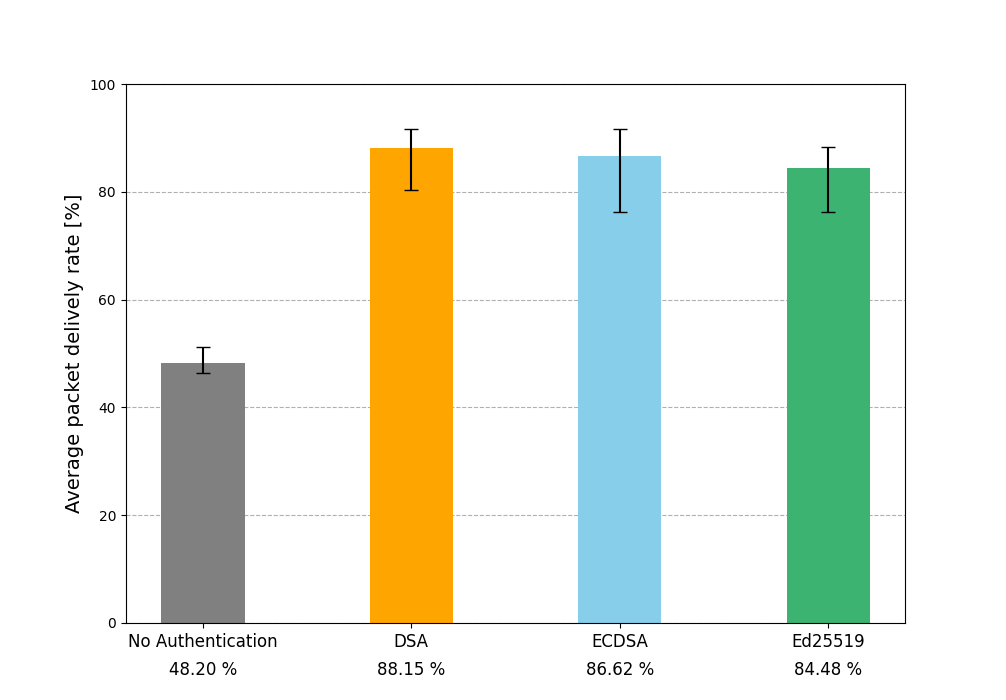
\includegraphics[width=1\textwidth]{figures/exp1_pdr.png}
  \caption{不正ノードが存在する環境でのパケット配送率}
  \label{fig:exp1_pdr}
\end{figure}
\clearpage
\begin{figure}
  \centering
  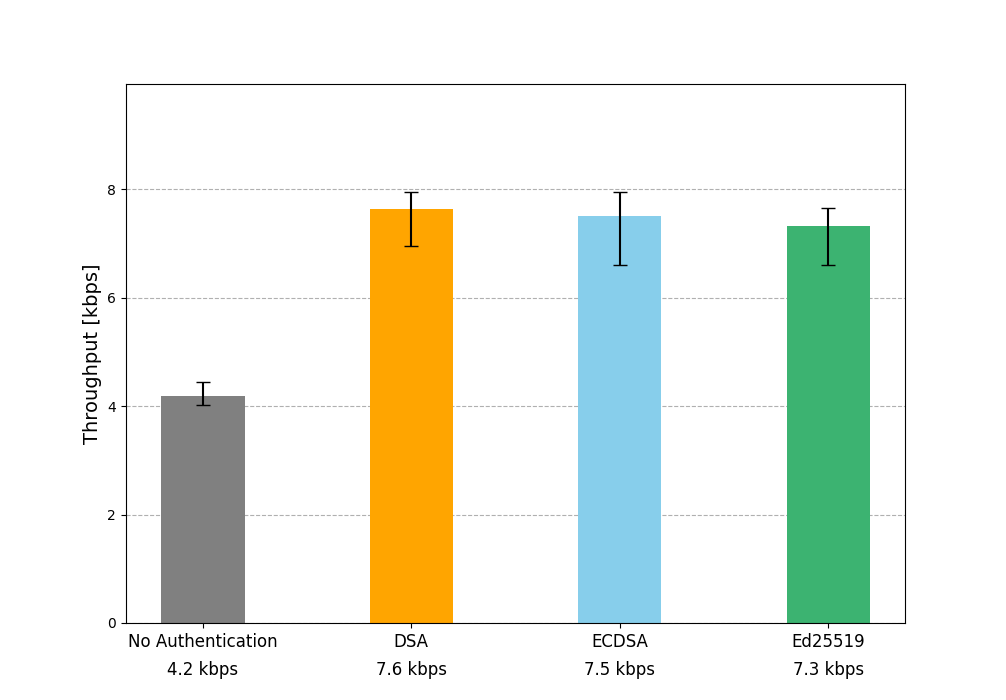
\includegraphics[width=1\textwidth]{figures/exp1_throughput.png}
  \caption{不正ノードが存在する環境でのスループット}
  \label{fig:exp1_throughput}
\end{figure}


\indent 図\ref{fig:exp1_pdr}は, 実験1におけるシミュレーションパターンごとの
パケット配送率を示している. 認証機構なしの場合に48.2 \%であるのに対し, 
ECDSAでは86.62 \%, EdDSAでは84.48 \%と, 認証機構を追加したことでパケット配送率が
約30 \%向上した. \\
\indent 図\ref{fig:exp1_throughput}は, 実験1におけるシミュレーションパターンごとの
スループットを示している. 認証機構なしの場合に4.18kbpsであるのに対し, 
ECDSAでは7.51kbps, EdDSAでは7.33kbpsと, 認証機構を
追加することでパケット配送率同様, スループットも向上した. \\
\indent これらの結果は, 認証機構の追加により 
不正ノードが排除されたことで, 経路選択を行う際に正当なノードのみが
選択されており,  データの窃取(転送中止)が回避できたことを示している. 
また, EdDSAの結果をECDSAの結果と比較するとほとんど差がないため, 
2つの署名方式が不正ノードを排除することにおいて同等のセキュリティ性能をもつと考えられる. 




\section{実験2}
実験2は認証機構の追加が通信にどれだけの負荷を与えるのかを
調査するための実験を行った. 
不正ノードの存在しない環境で, 250回シミュレーションを行い, 
遅延時間, 平均パケット配送率, オーバーヘッドサイズを調べた. \\
\indent 実験の結果は以下の通りである. \\

\begin{longtable}{ccc}
  \caption{遅延時間の中央値}
  \label{tab:exp2_delay} \\
  \endfirsthead
  \hline
  \multicolumn{1}{c}{プロトコル} &
  \multicolumn{1}{c}{中央値 [ms]} &
  \multicolumn{1}{c}{最頻値 [ms]} \\ \hline \hline
  No Authentication & $6.88$ & $[6.0, 7.0)$ \\
  DSA & $6.13$ & $[2.0, 3.0)$ \\
  ECDSA & $6.20$ & $[2.0, 3.0)$ \\
  Ed25519 & $6.42$ & $[6.0, 7.0)$ \\ \hline
\end{longtable}

\begin{figure}
  \centering
  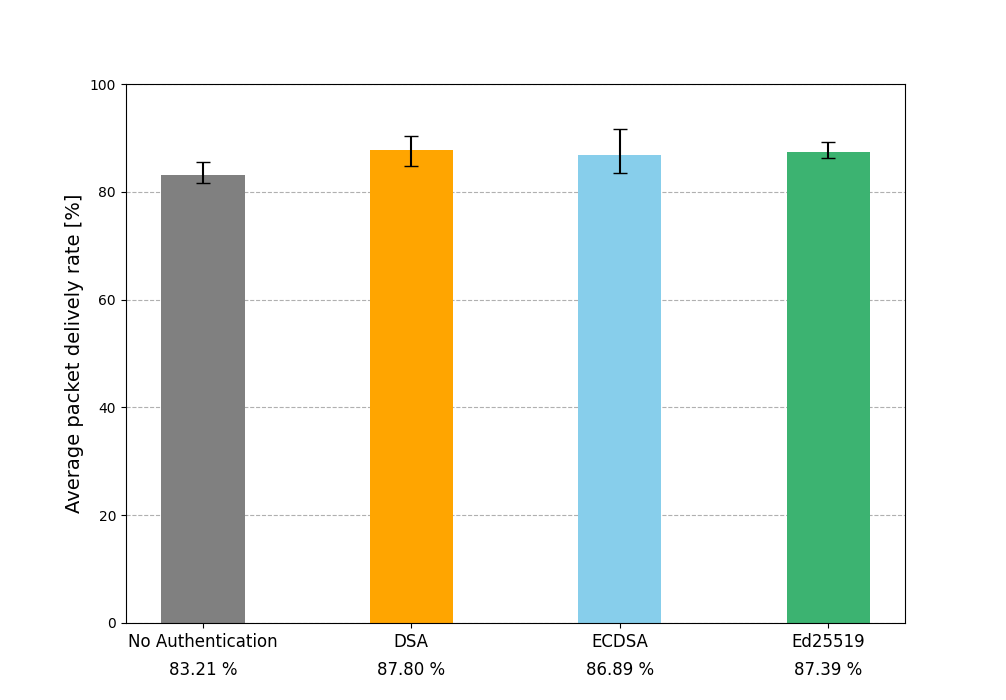
\includegraphics[width=1\textwidth]{figures/exp2_pdr.png}
  \caption{不正ノードが存在しない環境でのパケット配送率}
  \label{fig:exp2_pdr}
\end{figure}

\begin{figure}
  \centering
  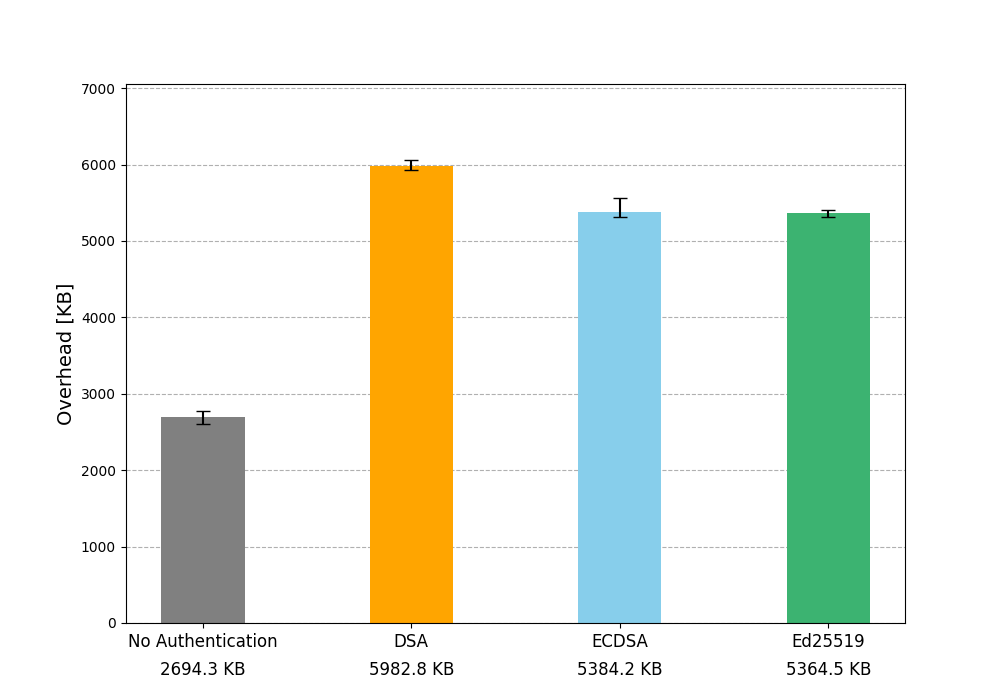
\includegraphics[width=1\textwidth]{figures/exp2_overhead.png}
  \caption{オーバーヘッドサイズ}
  \label{fig:exp2_overhead}
\end{figure}

\indent 表\ref{tab:exp2_delay}は, 実験2におけるシミュレーションパターンごとの
遅延時間の中央値と最頻値を示している. 中央値について, 認証機構なしでは6.88ms, 
DSAでは6.13ms, ECDSAでは6.2ms, EdDSAでは6.42msであった. 
最頻値について, 認証機構なしとEd25519では6.0msから7.0ms, 
DSAとECDSAでは2.0msから3.0msの範囲が最も多かった. 
この結果は, 遅延時間は経路選択のタイミングによって左右されるため, 
若干の差異が出てしまうが, 認証機構の有無が遅延時間に影響を与えなかったことを
示唆している. \\
\indent 図\ref{fig:exp2_pdr}は, 実験2におけるシミュレーションパターンごとの
平均パケット配送率を示している. 認証機構なしでは83.21 \%, DSAでは87.8 \%, 
ECDSAでは86.89 \%, EdDSAでは87.39 \%となった. この結果から, 
認証機構の有無はパケット配送率に影響を与えなかったと考えられる. \\
\indent 図\ref{fig:exp2_overhead}は, 実験2におけるシミュレーションパターンごとの
オーバーヘッドサイズを示している. 認証機構なしでは
2694.3KBであったのに対し, DSAでは5982.8KB, ECDSAでは5384.2KB, 
EdDSAでは5364.5KBと, 認証機構の追加により
オーバーヘッドサイズが大幅に増加した. これは, Helloパケットの
データに署名が付与されていることが原因である. また, 
EdDSAの結果をDSAとECDSAの結果と比較すると, EdDSAとDSAでは
大きな差があったのに対し, EdDSAとECDSAではほとんど差がなかった. 
EdDSAがDSAよりも鍵長が短いが, ECDSAとは変わらないことから
このような結果になったと考えられる. 
なお, 本研究で使用したパラメータによるそれぞれの鍵長は, 
DSAで2048ビット, ECDSAとEdDSAで256ビットである. \\



\section{実験3}
\indent 実験3では, 認証機構の処理能力(計算効率)を評価するための実験を行った. 
不正ノードの存在しない環境でノード数を37, 74, 112, 148, 185に設定して
250回ずつシミュレーションを行い, それぞれの実行にかかった時間を調べた.\\
\indent 実験の結果は以下の通りである. \\

\begin{figure}
  \centering
  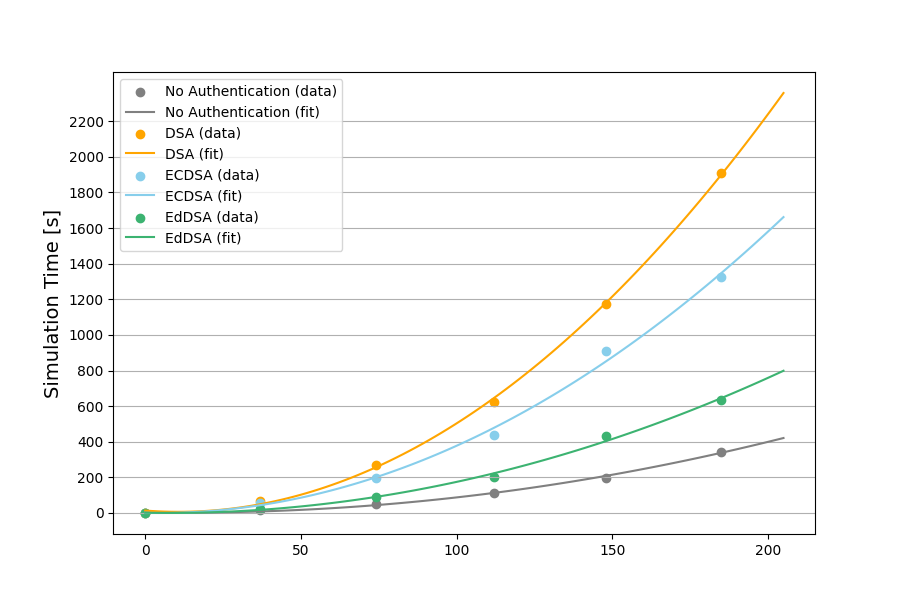
\includegraphics[width=1\textwidth]{figures/exp3_simtime.png}
  \caption{ノード数によるシミュレーション実行時間の変化}
  \label{fig:exp3_simtime}
\end{figure}

\setlength{\tabcolsep}{4pt}
\begin{longtable}{
    >{\raggedright\arraybackslash}p{3cm}
    >{\raggedright\arraybackslash}p{3.7cm}
    >{\raggedright\arraybackslash}p{2.5cm}
    >{\raggedright\arraybackslash}p{2.5cm}
    >{\raggedright\arraybackslash}p{2.5cm}
  }
  \caption{ノード数によるシミュレーション実行時間}
  \label{tab:exp3_simtime} \\
  \endfirsthead
  \hline
  % \multicolumn{1}{c}{Number of nodes} &
  % \multicolumn{1}{c}{No Authentication [s]} &
  % \multicolumn{1}{c}{DSA [s]} &
  % \multicolumn{1}{c}{ECDSA [s]} &
  % \multicolumn{1}{c}{Ed25519 [s]} \\ \hline \hline
  Number of nodes & No Authentication $[s]$ & DSA $[s]$ & ECDSA $[s]$ & Ed25519 $[s]$ \\ \hline \hline
  \multicolumn{1}{c}{$37$} &
  \multicolumn{1}{c}{$14.1802$} &
  \multicolumn{1}{l}{$69.9882$} &
  \multicolumn{1}{l}{$55.0108$} &
  \multicolumn{1}{l}{$24.4069$} \\
  \multicolumn{1}{c}{$74$} &
  \multicolumn{1}{c}{$50.5984$} &
  \multicolumn{1}{l}{$267.433$} &
  \multicolumn{1}{l}{$194.408$} &
  \multicolumn{1}{l}{$89.2728$} \\
  \multicolumn{1}{c}{$112$} &
  \multicolumn{1}{c}{$110.405$} &
  \multicolumn{1}{l}{$625.504$} &
  \multicolumn{1}{l}{$436.926$} &
  \multicolumn{1}{l}{$200.901$} \\
  \multicolumn{1}{c}{$148$} &
  \multicolumn{1}{c}{$196.971$} &
  \multicolumn{1}{l}{$1172.57$} &
  \multicolumn{1}{l}{$910.373$} &
  \multicolumn{1}{l}{$431.346$} \\
  \multicolumn{1}{c}{$185$} &
  \multicolumn{1}{c}{$345.059$} &
  \multicolumn{1}{l}{$1908.7$} &
  \multicolumn{1}{l}{$1324.55$} &
  \multicolumn{1}{l}{$635.155$} \\ \hline

  % $37$ & $14.1802$ & $69.9882$ & $55.0108$ & $24.4069$ \\
  % $74$ & $50.5984$ & $267.433$ & $194.408$ & $89.2728$ \\
  % $112$ & $110.405$ & $625.504$ & $436.926$ & $200.901$ \\
  % $148$ & $196.971$ & $1172.57$ & $910.373$ & $431.346$ \\
  % $185$ & $345.059$ & $1908.7$ & $1324.55$ & $635.155$ \\ \hline
\end{longtable}

\begin{longtable}{ccc}
  \caption{1回の署名作成と署名検証にかかった時間}
  \label{tab:exp3_sigtime} \\
  \endfirsthead
  \hline
  \multicolumn{1}{c}{プロトコル} &
  \multicolumn{1}{c}{署名作成時間 $[\mu s]$} &
  \multicolumn{1}{c}{署名検証時間 $[\mu s]$} \\ \hline \hline
  ECDSA & $371.020$ & $336.938$ \\
  Ed25519 & $31.349$ & $97.036$ \\ \hline
\end{longtable}

\indent 図\ref{fig:exp3_simtime}はシミュレーションパターンごとのノード数による
実行時間の変化を近似してグラフ化したものを, 表\ref{tab:exp3_simtime}はその具体的な
値を示したものである. さらに, 表\ref{tab:exp3_sigtime}にはECDSAとEdDSAにおいて, 1回の署名作成と
署名検証にかかった時間を示した. \\
\indent 図\ref{fig:exp3_simtime}, 表\ref{tab:exp3_sigtime}より, 
EdDSA, ECDSA, DSAの順番で実行時間が短いのがわかる. また, 
表\ref{tab:exp3_sigtime}に示すように, EdDSAがECDSAに比べて
署名生成, 署名検証にかかる時間が短いことから, EdDSAは
3つの署名方式の中で最も計算効率が良いということが確かめられた. 
さらに, ECDSAとEdDSAの計算効率の差はノード数が増加するほど, 
実行時間全体に与える影響が大きなっており, EdDSAが
よりスケーラビリティに優れていることを示唆している. 